% LOPUT:

%\begin{enumerate}
%\item
%Olkoot $A(x)$ avoin lause ''paikkakunnalla $x$ paistaa
%aurinko'' ja $T(x)$ avoin lause ''paikkakunnalla $x$
%tuulee''. Suomenna lause.
%\begin{enumerate}[a)]
%\item $\lnot T(x)$,
%\item $A(x) \land T(y)$,
%\item $\lnot A(\textrm{Lempäälä})$,
%\item $\lnot (A(\textrm{Turku}) \to T(\textrm{Kuopio}))$.
%\end{enumerate}%

%\item
%Olkoot $S(x)$ avoin lause ''$x$ on suomalainen
%formulakuljettaja'' ja $E(x)$ avoin lause ''$x$ on
%eurooppalainen formulakuljettaja, joka ei ole
%suomalainen''. Kuljettaja voi olla joko nykyinen tai
%entinen. Ratkaise avoin lause, kun perusjoukko on
%$\{\textrm{Räikkönen}, \textrm{Vettel}, \textrm{Senna}\}$.
%\begin{enumerate}[a)]
%\item $S(x)$,
%\item $\lnot S(x)$,
%\item $E(x)$,
%\item $\lnot (S(x) \lor E(x))$.
%\end{enumerate}%

%\item
%Olkoon $Q(x)$ avoin lause ''$x^2 = 64$''. Onko lause a)
%$Q(-8)$ b) $Q(6)$ tosi?%

%\item
%Olkoon $P(x, y)$ avoin lause ''$x^2 + y \le 0$''. Onko
%lause a) $P(0, 0)$ b) $P(-1, 1)$ c) $P(5, -100)$ tosi?%

%\item
%Olkoot $S(x)$ avoin lause ''kuvio $x$ on symmetrinen
%jonkin suoran suhteen'' ja $P(x)$ avoin lause ''kuvio $x$
%on symmetrinen jonkin pisteen suhteen''. Perusjoukon
%muodostavat oheiset kuviot. Ratkaise avoin lause.
%\begin{enumerate}[a)]
%\item $S(x)$,
%\item $P(x)$,
%\item $\lnot (S(x) \lor P(x))$,
%\item $S(x) \lequiv P(x)$.
%\end{enumerate}%

%\begin{center}
%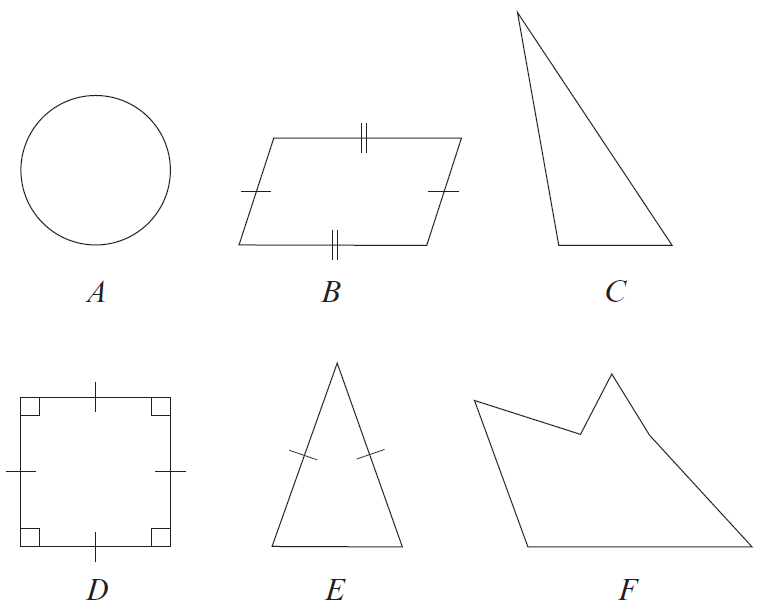
\includegraphics[width=10cm]{pictures/kpl3_2_teht7}
%\end{center}%

%\item
%Ratkaise avoin lause $4x^2 + 7x - 2 = 0$, kun perusjoukko
%on a) reaalilukujen joukko b) kokonaislukujen joukko.%

%\item
%Olkoot perusjoukko $\{ 0, 1, 2, \ldots , 10\}$, $A(x)$
%avoin lause ''$x \le 1$'' ja $B(x)$ avoin lause ''$x > 5$''.
%Ratkaise avoin lause.
%\begin{enumerate}[a)]
%\item $A(x)$,
%\item $\lnot B(x)$,
%\item $A(x) \land B(x)$,
%\item $\lnot A(x) \to B(x)$.
%\end{enumerate}%

%\item
%Arvotaan kaksi lukua, joista molemmat voivat olla 1, 2 tai 3. Arvonnan tuloksena saadaan lukupari $(x, y)$, missä $x$ on ensimmäisen arvonnan tulos ja $y$ toisen arvonnan tulos. Olkoot avoimet lauseet $S(x, y)$: ''$x \le y$'' ja $T(x, y)$: ''tulo $xy$ on jaollinen luvulla 3''. Ratkaise avoin lause, kun perusjoukon muodostavat arvonnan tuloksena saatavat mahdolliset lukuparit
%\[
%(1, 1),\ (1, 2),\ (1, 3),\ (2, 1),\ (2, 2),\ (2, 3),\ (3, 1),\ (3, 2),\ (3, 3).
%\]
%\begin{enumerate}[a)]
%\item $S(x, y)$,
%\item $\lnot T(x, y)$,
%\item $\lnot (S(x, y) \lor T(x, y))$,
%\item $S(x, y) \to T(x, y)$.
%\end{enumerate}%

%\item
%Ratkaise reaalilukujen joukossa
%\begin{enumerate}[a)]
%\item epäyhtälö $x^2 \le 4$,
%\item epäyhtälöpari
%\[
%\left\{
%\begin{array}{rcl}
%x^2 & \le & 4 \\
%x & > & -1.
%\end{array}\right.
%\]
%\end{enumerate}%

%\item
%Ratkaise reaalilukujen joukossa epäyhtälö
%\begin{enumerate}[a)]
%\item $|x| > 5$,
%\item $|x| \le 1$,
%\item $|x - 4| > 5$,
%\item $|2x - 6| \le 1$.
%\end{enumerate}%

%\item Ratkaise avoin lause reaalilukujen joukossa. Ilmaise ratkaisujoukko myös välimerkintää käyttäen.
%\begin{enumerate}[a)]
%\item $(x^2 > 1) \lor (0 \le x \le 2)$,
%\item $(x^2 > 1) \land (0 \le x \le 2)$,
%\item $(x^2 > 1) \to (0 \le x \le 2)$.
%\end{enumerate}%

%\item
%Olkoot $P(x)$ avoin lause $(x < 10) \land (x^2 = 100)$ ja
%$Q(x)$ avoin lause $(x \ge 10) \lequiv (x^2 = 100)$. Ratkaise avoin lause reaalilukujen joukossa.
%\begin{enumerate}[a)]
%\item $P(x)$,
%\item $Q(x)$,
%\item $P(x) \lor Q(x)$,
%\item $P(x) \land Q(x)$.
%\end{enumerate}%
%

%\end{enumerate}%

%\subsection*{Kotitehtäviä}%

%\begin{enumerate}%

%\item
%Olkoon $T(x, y)$ avoin lause ''$x$ lähettää tekstiviestin
%$y$:lle''. Suomenna lause.
%\begin{enumerate}[a)]
%\item $T(\textrm{Tiina}, \textrm{Elias})$,
%\item $\lnot T(\textrm{Elias}, \textrm{Tiina}) \land T(\textrm{Elias}, \textrm{Vilma})$,
%\item $T(x, x)$,
%\item $T(y, \textrm{Rasmus}) \lequiv T(\textrm{Rasmus}, y)$.
%\end{enumerate}%

%\item
%Olkoot $E(x)$ avoin lause ''$x$ on eurooppalainen
%pääkaupunki'' ja $S(x)$ avoin lause ''$x$ on suomalainen
%kaupunki''. Ratkaise avoin lause, kun perusjoukko on
%$\{\textrm{Helsinki}, \textrm{Rovaniemi}, \textrm{Praha}, \textrm{Milano}\}$.
%\begin{enumerate}[a)]
%\item $E(x)$,
%\item $\lnot S(x)$,
%\item $S(x) \land \lnot E(x)$,
%\item $\lnot (E(x) \land S(x))$,
%\item $E(x) \lequiv S(x)$.
%\end{enumerate}%

%\item
%Olkoon $R(x)$ avoin lause ''$x^2 - 100 > 0$''. Onko lause
%a) $R(10)$ b) $R(-15)$ tosi?%

%\item
%Olkoon $S(x, y)$ avoin lause ''$x^2 + y^2 = 5$''. Onko
%lause a) $S(2, 3)$ b) $S(2, -1)$ c) $S(-\sqrt{5}, 0)$ d)
%$S(-1, -1)$ tosi?%

%\item
%Ratkaise avoin lause $9x^2 + 30x + 25 \le 0$, kun
%määrittelyjoukko on a) reaalilukujen joukko b)
%kokonaislukujen joukko.%

%\item
%Olkoot perusjoukko $\{ 1, 2, 3, \ldots , 16\}$, $C(x)$
%avoin lause ''luku 12 on jaollinen luvulla $x$'' ja $D(x)$ avoin lause ''luvun $x$ neliöjuuri on kokonaisluku''.
%Ratkaise avoin lause.
%\begin{enumerate}[a)]
%\item $C(x)$,
%\item $D(x)$,
%\item $\lnot C(x) \land D(x)$,
%\item $C(x) \lequiv D(x)$.
%\end{enumerate}%

%\item
%Arvotaan kolme lukua, joista jokainen voi olla 1 tai
%2. Arvonnan tuloksena saadaan lukukolmikko $(x, y, z)$, missä $x$ on ensimmäisen arvonnan tulos, $y$ toisen arvonnan tulos ja $z$ kolmannen arvonnan tulos. Olkoot
%avoimet lauseet $S(x, y, z)$: ''$x + y + z \ge 5$'', $T(x,
%y, z)$: ''tulo $xyz$ on pariton'' ja $U(x, y, z)$: “summa
%$x + y + z$ on jaollinen luvulla 3''. Ratkaise avoin
%lause, kun perusjoukon muodostavat arvonnan tuloksena
%saatavat mahdolliset lukukolmikot
%\[
%(1, 1, 1),\ (1, 1, 2),\ (1, 2, 1),\ (1, 2, 2),\ (2, 1, 1),\ (2, 1, 2),\ (2, 2, 1),\ (2, 2, 2).
%\]
%\begin{enumerate}[a)]
%\item $S(x, y, z)$,
%\item $T(x, y, z)$,
%\item $U(x, y, z)$,
%\item $S(x, y, z) \land T(x, y, z)$,
%\item $S(x, y, z) \lor \lnot U(x, y, z)$,
%\item $\lnot (S(x, y, z) \lor T(x, y, z) \lor U(x, y, z))$,
%\item $S(x, y, z) \land (T(x, y, z) \lequiv U(x, y, z))$.
%\end{enumerate}%

%\item
%Ratkaise reaalilukujen joukossa.
%\begin{enumerate}[a)]
%\item $x^2 = 1$ tai $x(x + 5)(x - 1) = 0$
%\item $x^2 = 1$ ja $x(x + 5)(x - 1) = 0$
%\end{enumerate}%

%\item
%Ratkaise reaalilukujen joukossa
%\begin{enumerate}[a)]
%\item epäyhtälö $x^2 - 11x + 30 > 0$,
%\item epäyhtälöpari
%\[
%\left\{
%\begin{array}{rcl}
%x^2 - 11x + 30 & > & 0 \\
%2x & > & -6 - x.
%\end{array}\right.
%\]
%\end{enumerate}%

%\item Ratkaise avoin lause reaalilukujen joukossa. Ilmaise ratkaisujoukko myös välimerkintää käyttäen.
%\begin{enumerate}[a)]
%\item $(-4 < x) \lor (x < 8)$,
%\item $(-4 < x) \land (x < 8)$,
%\item $((-4 < x) \land (x < 8)) \land (-5 \le x \le -3)$,
%\item $(-4 < x) \lequiv (-5 \le x \le -3)$.
%\end{enumerate}%

%\item
%Olkoot $A(x)$ avoin lause $(x \ge 0) \to (x \ge 20)$
%ja $B(x)$ avoin lause $\lnot ((x \le 0) \lor (x \ge 20))$. Ratkaise avoin lause reaalilukujen joukossa.
%\begin{enumerate}[a)]
%\item $A(x)$,
%\item $B(x)$,
%\item $A(x) \lor B(x)$.
%\end{enumerate}
